%
% Spectral tomography of multi-photon states
%
% Keith R. Motes, Ben Baraglioa, Alexei Gilchrist, Joshua Combes, Peter P. Rohde
% Macquarie University, University of New Mexico
%
% July 2013
%

\documentclass[aps,pra,twocolumn,amsmath,amssymb,color,superscriptaddress]{revtex4}

\usepackage[pdftex]{graphicx}
\usepackage{mathrsfs}
\usepackage[usenames,dvipsnames]{color}
\usepackage[colorlinks]{hyperref}

\newcommand{\bra}[1]{\langle#1|}
\newcommand{\ket}[1]{|#1\rangle}
\newcommand{\op}[2]{\hat{\textbf{#1}}_{#2}}
\newcommand{\dagop}[2]{\hat{\textbf{#1}}_{#2}^\dag}
\newcommand{\ip}[2]{\langle{#1}|{#2}\rangle} %inner product
\newcommand{\outp}[2]{\ket{#1}\bra{#2}}     %outerproduct
\newcommand{\expt}[1]{\langle{#1}\rangle}
\newcommand{\dg}{^\dagger}
\newcommand{\erf}[1]{Eq.~(\ref{#1})}
\newcommand{\Id}{I}

\newcommand{\red}{\color{red}}
\newcommand{\blue}{\color{blue}}
\newcommand{\green}{\color{ForestGreen}}
\newcommand{\purple}{\color{RoyalPurple}}

\begin{document}

\bibliographystyle{apsrev}

%
% Title & authors
%

\title{Photo counting distributions of multi-photon states by time resolved photo-detection}
%\title{Spectral tomography of multi-photon states}

\author{Keith R. Motes}
\affiliation{Centre for Engineered Quantum Systems, Department of Physics and Astronomy, Macquarie University, Sydney NSW 2113, Australia}

\author{Ben Baragiola}
\affiliation{Center for Quantum Information and control, University of New Mexico, Albuquerque, NM 87131-0001, USA}

\author{Alexei Gilchrist}
\affiliation{Centre for Engineered Quantum Systems, Department of Physics and Astronomy, Macquarie University, Sydney NSW 2113, Australia}

\author{\blue Joshua Combes}
\affiliation{Center for Quantum Information and control, University of New Mexico, Albuquerque, NM 87131-0001, USA}

\author{Peter P. Rohde}
\email[]{dr.rohde@gmail.com}
\homepage{http://www.peterrohde.org}
\affiliation{Centre for Engineered Quantum Systems, Department of Physics and Astronomy, Macquarie University, Sydney NSW 2113, Australia}

\date{\today}

\frenchspacing

%
% Abstract
%

\begin{abstract}
Photons exhibit a rich spectral structure, which is highly relevant when considering interference effects between photonic states. Thus, tomographically reconstructing the spectral structure of photonic states is of great interest. We describe a tomographic procedure for reconstructing the spectral structure of multi-photon states using a Bayesian algorithm. The algorithm utilises the known temporal response of the photo-detectors to perform the reconstruction. We find that in the limit of fast detectors a perfect reconstruction is possible, whereas for slow detectors the reconstruction is limited by the response time of the detectors. The described Bayesian reconstruction algorithm improves the inferred spectral structure compared to the raw measurement statistics.\\
{\blue (1)  $\hat a$\\ 
(2) $dt$ {\bf and} $\int .... dt$ \\ 
(3) we need a notational way of distinguishing between Fock states and $n$-photon states. I will adopt the following convention $\ket{n_\psi}$ is a Fock state and $\ket{\psi_n}$ is an $n$-photon state. Feel free to come up with something better.\\ (4) remind me, what is the norm convention we decided on for $n$-photon states. Should the TDF have a $(n!)^2$ or not? }
\end{abstract}

\maketitle

%
% Introduction
%

\section{Introduction}

Photonic states are typically considered in the photon number (Fock) basis. However, photons also exhibit a rich spectral/temporal structure \cite{bib:RohdeMauererSilberhorn07}, which is highly relevant in many optical quantum information processing tasks \cite{bib:NielsenChuang00, bib:KokLovett11}. For example: the spectral structure of states prepared via parametric down-conversion (PDC) strongly affects the purity of heralded photons \cite{bib:Rubin94, bib:URen05}; the differences between the spectral structure of two photons will affect their interference properties at a beamsplitter, the well known Hong-Ou-Mandel (HOM) effect \cite{bib:HOM87}; and, in optical quantum information processing schemes, the spectral structure of photons affects the fidelity of gate operations \cite{bib:RohdeRalph05, bib:RohdeRalph05b, bib:RohdeRalph06, bib:RohdeRalphMunro06}. Thus, characterising the spectral structure of photons is of great interest in many applications, motivating the desire to perform spectral tomography on photonic states \cite{bib:Rohde06b}.

We describe a Bayesian technique for tomographically reconstructing the spectral structure of a multi-photon state using a physically realistic model for time-resolved photo-detection. The technique combines \emph{a priori} knowledge of the temporal response of the detectors with measurement statistics using a Bayesian algorithm. We find that in the limit of good detectors (fast response time) a perfect reconstruction of the temporal distribution function (TDF) is possible, whereas as the response of the detectors becomes slower the quality of the reconstruction is reduced. The Bayesian approach yields an advantage over the raw measurement data.

%
% The spectral structure of photons
%

\section{The spectral structure of photons}

Typically, quantum opticians represent photonic states in the photon number (Fock) basis. An $n$-photon state in one mode would be expressed as the $n$th power of the photon creation operator,
\begin{equation}
\ket{n} = \frac{1}{\sqrt{n!}}(a^\dag)^n {\blue \ket{0}}.
\end{equation}
{\blue This single mode description, i.e. $[a,a\dg]=1$, is appropriate for a single mode cavity. However, to describe traveling or itinerant photons requires multiple modes. Multimode-photons can exhibit spectral/temporal and spatial structure that is not present in there single mode counterparts. In what follows we use continuous-mode quantized field operators within the quasi-monochromatic approximation \cite{BlowLoudon}. In this framework the commutation relations are those of white noise $[a(t),a\dg(s)]= \delta(t-s)$.} Consequently the temporal structure of a single photon state can be expressed as,
\begin{equation}\label{onephoton}
\ket{1_\psi} \equiv A^\dag_{\psi(t)}\ket{0} = \int \psi(t)a^\dag(t) \,dt\ket{0},
\end{equation}
where $A^\dag_{\psi(t)}$ is a mode operator that creates a photon with a {\blue temporal-distribuiton function (TDF) given by \mbox{$\psi(t)$}  \cite{bib:RohdeMauererSilberhorn07,BlowLoudon}. The spectral distribution function (SDF), $\tilde\psi(\omega)$, is easily obtained via the Fourier transform. Then a Fock state, where each photon photon exhibit identical temporal structure i.e. $\psi(t)$, can be expressed as the $n$th power of the mode operator. We will denote a general Fock state as $\ket{n_\psi}$. But there exist states with a definite number of photons that also exhibit temporal/spectral correlations. We call such states $n$-photon states and denote them by $\ket{\psi_n}$. The most general form of an $n$-photon states is}
\begin{equation}
\ket{\psi_n} = \int \!\! \dots \!\! \int \psi_n(t_1,\dots,t_n) \hat{a}^\dag(t_1) \dots \hat{a}^\dag(t_n)\,dt_1\dots dt_n \ket{0},
\end{equation}
where \mbox{$\psi(t_1,\dots,t_n)$} is the joint TDF of the multi-photon state in a single spatial mode, and $\hat{a}^\dag(t)$ is the photon creation operator at time $t$. This formalism also extends to multi-mode states. For example, an $n$-photon state with exactly one photon per mode could most generally be expressed as,
\begin{equation} \label{eq:multi_mode}
\ket{\psi_n} = \int \!\! \dots \!\! \int \psi_n(t_1,\dots,t_n) \hat{a}_1^\dag(t_1) \dots \hat{a}_n^\dag(t_n)\,dt_1\dots dt_n \ket{0},
\end{equation}
where $a_i^\dag$ is the photon creation operator for the $i$th mode. We refer the reader to Rohde \emph{et al.} \cite{bib:RohdeMauererSilberhorn07} for a rigorous treatment of the temporal/spectral structure of photons. {\blue Should we cite related work by Oh ?}

%
% Time-resolved photo-detection
%
\section{Time-resolved photo-detection} \label{sec:det_model}
In this section we describe the theory of Time-resolved photo-detection. We start by describing the abstract quantum measurement theory of an idealized theory of a detector with infinite temporal resolution. Next we show how to model the finite time resolution of actual detectors by convolving the idealized detector with a probability distribution which represents the detector response to a incident photon. The detector response function is obtained through detector tomography.
 
 \subsection{idealized time-resolved detection}
Photon counting in an infinitesimal time interval only the presence or absence of a photon can be detected. That is, the time interval is chosen small enough so the probability of detecting two photons is negligible; other situations can be obtained by a suitable coarse graining. Thus, the projectors that describe infinitesimal photon counting measurements need only resolve the identity on this restricted Fock space at every time \cite{JackCollett}. We define the photon counting projectors over the interval $[t,t + dt)$ to be
\begin{subequations}\label{eq:projectors}
\begin{align} 
		\Pi_0 (t) = & \Id_{[0,t)}\otimes \outp{0}{0} \otimes \Id_{[t+dt,\infty)}\\
		\Pi_1(t)                 = & \Id_{[0,t)}\otimes \outp{1}{1} \otimes \Id_{[t+dt,\infty)},
\end{align}
\end{subequations}
where the one photon projection is onto the square wave packet
\begin{align}\label{eq:InfinitesimalState}
		\ket{1}= \frac{1}{\sqrt{dt}}  \int_{t}^{t+dt} ds\, a^\dagger (s) \ket{0} .
\end{align}
Using the projectors in \erf{eq:projectors} one can calculate the probabilities for detecting vacuum or a single photon in the time interval $[t,t + dt)$ for the state in \erf{onephoton} 
\begin{subequations}\label{asdf}
\begin{align} 
\Pr(0|\psi) &= \bra{1_\psi} \Pi_0 (t)\ket{1_\psi}= 1-dt|\psi(t)|^2,\\
\Pr(1|\psi) &= \bra{1_\psi} \Pi_1 (t)\ket{1_\psi}= dt|\psi(t)|^2.
\end{align}
\end{subequations}
Notice how the probability for a count is proportional to the infinitesimal $dt$, thus the probability for two counts is proportional to the square of the infinitesimal which is formally zero.

For more than one photon we are generally interested in the distribution of click times. For Fock states the distribution of the click times is identical for all photons. For $n$-photon states the count distribution is    
\begin{align}
p(t_1,t_2,t_3, \ldots, t_N|\psi_n) = (n!)^2   |\psi\big(t_1,t_3,t_3,\ldots, t_n \big)|^2,
\end{align}
as shown in appendix \ref{derivation}. Using Bayes rule


 \subsection{realistic time-resolved detection}

{\blue ============ up to here ============}\\
The classical probability distribution {\blue of the photon count times} is given by the absolute square of the TDF,
\begin{equation}
P_S(t_1,\dots,t_n|\psi_n)=|\psi(t_1,\dots,t_n)|^2.
\end{equation}

We model the photo-detectors as two-level systems which couple to the incident light, as employed by Metz \& Barrett \cite{bib:metz2008effect}. An incident photon excites the atom from the lower (ready) to the upper (triggered) level. Upon relaxation, the atom emits a photon which is detected by an ideal photo-detector. Thus, the two-level system acts as a buffer between the measured state and the detection process. The relaxation time of the atom determines the temporal resolving power of the detector. In the limit of a fast detector (i.e. quick relaxation time) the detector has delta function response, giving us perfect information about the measurement time of the detected photon, whereas for a slow detector the response is flat, yielding little information about the measurement time. The detector model is illustrated in Fig.~\ref{fig:det_model}.

\begin{figure}[!htb]
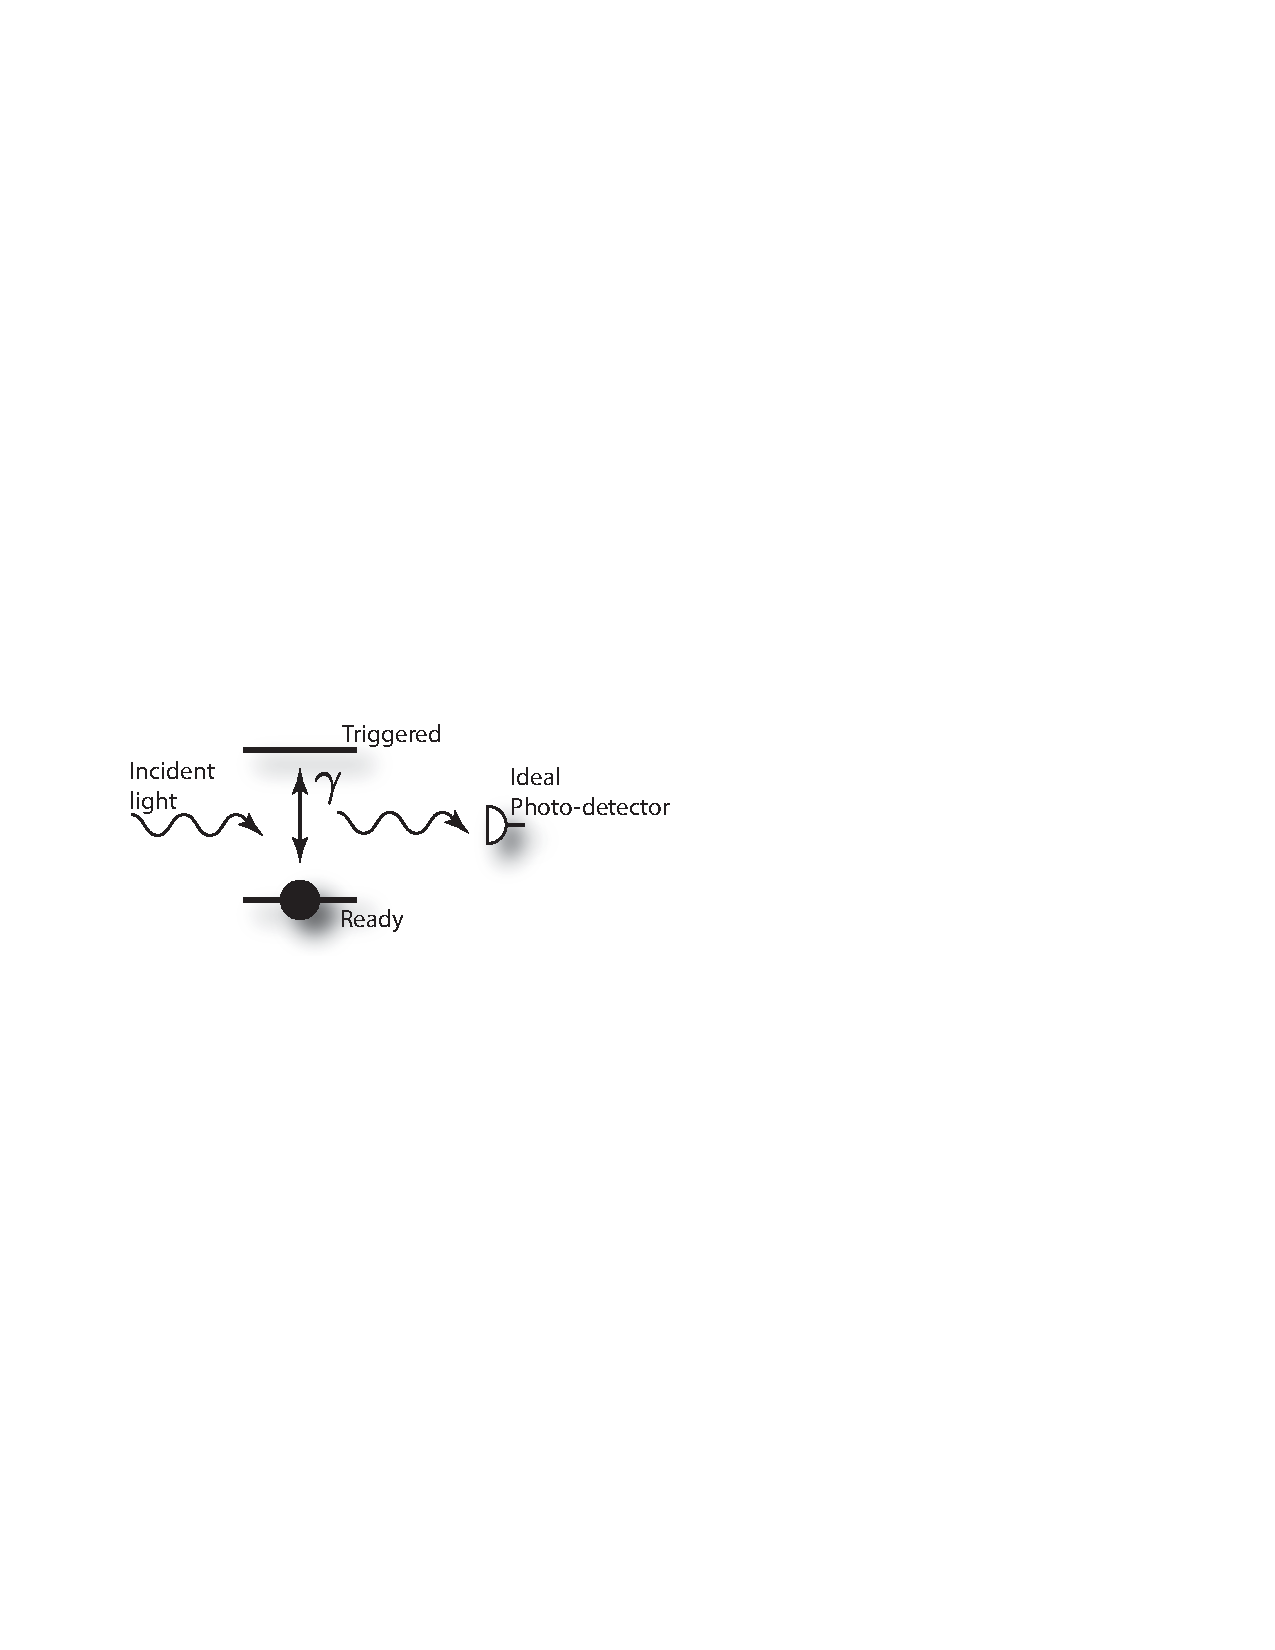
\includegraphics[width=0.7\columnwidth]{../figures/detector_model}
\caption{Model for a time-resolved photo-detector. The incident light couples two a two-level system, stimulating it from the `ready' to the `triggered' state. The two-level system then relaxes and the emitted photon is measured. Thus, the two-level system acts as a buffer between the measured state and the measurement circuitry. The relaxation time $\gamma$ of the two-level system determines the detector's time resolution.} \label{fig:det_model}
\end{figure}

The decay rate of this two-level system can be modelled as \cite{bib:loudon2000quantum},
\begin{equation}
N(t)=e^{-\gamma t}, \,\, t\geq 0,
\end{equation}
where $N(t)$ is the probability that the system is in the excited state at time $t$, and $\gamma$ is the relaxation rate (small $\gamma$ corresponds to a slow relaxation time and large $\gamma$ to a fast relaxation time). This two-level system couples to an ideal time-resolving photo-detector. From this one can calculate the conditional probability that the detector clicks at time $m$ given that the incident photon arrived at time $t$,
\begin{equation}
   P_D(m|t)=  \left\{
     \begin{array}{lr}
       0 & m < t \\
       \beta(\gamma) e^{-\gamma(t-m)} & m \geq t
     \end{array},
   \right.
\end{equation}
where $\gamma$ now takes the role of the response time of the detector and $\beta(\gamma)$ is a normalisation factor. \mbox{$P_D(m|t)=0$} for \mbox{$m<t$} because the photon cannot have arrived after the detector clicked. 

The response function for this detector model is illustrated in Fig.~\ref{fig:detector_response} for varying response times, $\gamma$. Small $\gamma$ corresponds to a slow detector, and large $\gamma$ to a fast detector.
\begin{figure}[!htb]
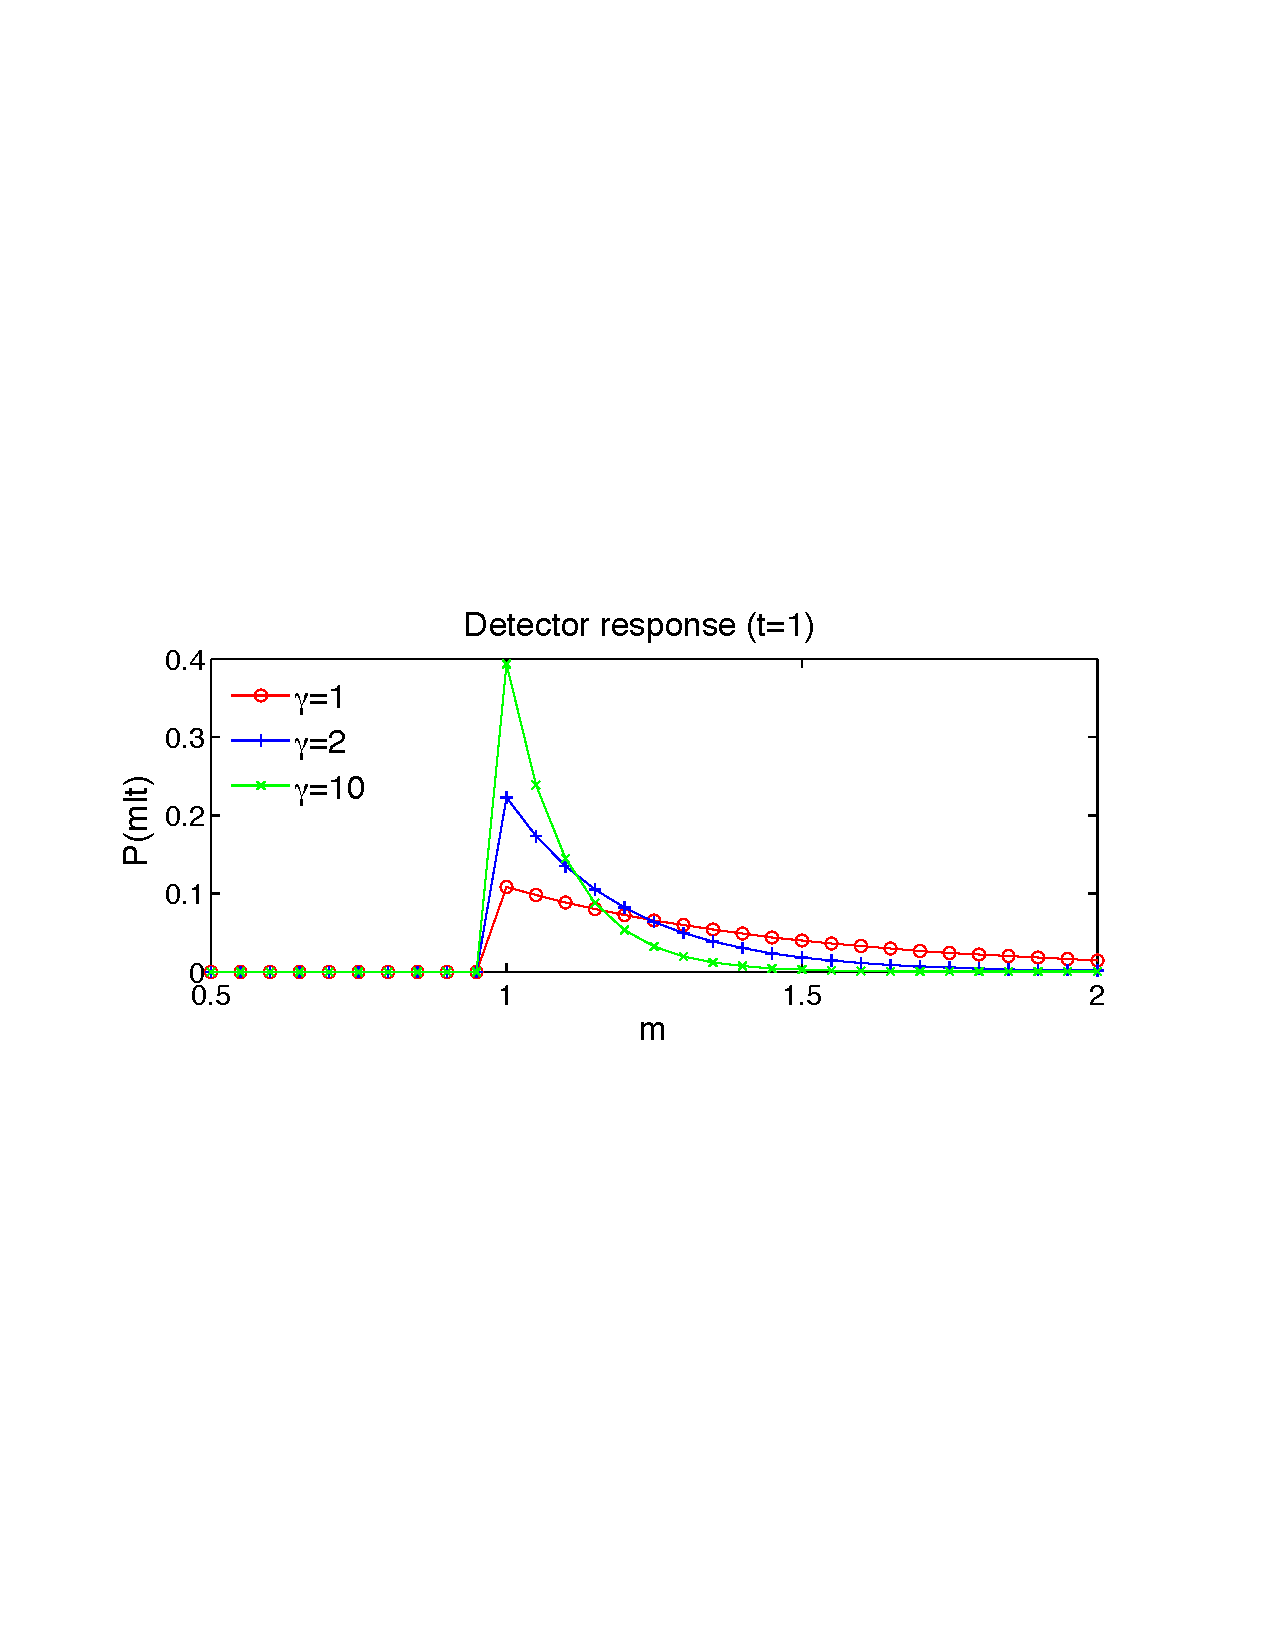
\includegraphics[width=\columnwidth]{../figures/detector_response}
\caption{(Colour online) Response function for a time-resolved detector with different response times, $\gamma$.} \label{fig:detector_response}
\end{figure}

%
% POVM description for time-resolved photo-detection
%

\subsection{POVM description for time-resolved photo-detection}

For a time-resolved detector characterised by the response function $P_D(m|t)$ we can explicitly formulate the POVM \cite{bib:NielsenChuang00} description. For the single-photon measurement outcome $m$, the associated POVM element is,
\begin{equation}
\hat\Pi(m) = \int P_D(m|t) \hat{a}^\dag(t) \ket{0}\bra{0} \hat{a}(t) \, \mathrm{d}t.
\end{equation}
It can easily be verified that $\hat\Pi(m)$ forms a POVM. First, the POVM elements add to unity,
\begin{eqnarray}
\int \hat\Pi(m) \, \mathrm{d}m &=& \int\!\!\int P_D(m|t) \hat{a}^\dag(t) \ket{0}\bra{0} \hat{a}(t) \, \mathrm{d}t\, \mathrm{d}m \nonumber\\
&=& \int \left(\int P_D(m|t) \,\mathrm{d}m\right) \hat{a}^\dag(t) \ket{0}\bra{0} \hat{a}(t)\, \mathrm{d}t \nonumber \\
&=& \int \hat{a}^\dag(t) \ket{0}\bra{0} \hat{a}(t)\, \mathrm{d}t \nonumber \\
&=& \hat{I}.
\end{eqnarray}
Second, $\bra{\psi}\hat\Pi(m)\ket{\psi}=P_M(m)$, where $P_M(m)$ is the measurement's expectation value. Let,
\begin{equation}
\ket\psi = \int \psi(t) \hat{a}^\dag(t)\,\mathrm{d}t \ket{0},
\end{equation}
be a single-photon wavepacket. Then,
\begin{eqnarray} \label{eq:PM_single_photon}
P_M(m) &=& \bra{\psi}\hat\Pi(m)\ket{\psi} \nonumber \\
&=& \int |\psi(t)|^2 P_D(m|t)\,\mathrm{d}t,
\end{eqnarray}
which is the expectation value of sampling the classical distribution $|\psi(t)|^2$ with a detector characterised by $P_D(m|t)$.

In the case of an $n$-mode measurement with one photon per mode, we apply the POVM to each mode and the measurement expectation values are given by,
\begin{eqnarray}
&&E(m_1,\dots,m_n) = \bra{\psi} \hat\Pi(m_1) \otimes \dots \otimes \hat\Pi(m_n) \ket{\psi} \nonumber \\
&&= \int \!\! \dots \!\! \int |\psi(t_1,\dots,t_n)|^2 \prod_{i=1}^n P_D(m_i|t_i)\,\mathrm{d}t_1\dots\mathrm{d}t_n. \nonumber\\
\end{eqnarray}

A time- and number-resolved detector on a single mode is easily generalised as,
\begin{eqnarray}
&&\hat\Pi(m_1,\dots,m_n) = \int \!\! \dots \!\! \int P_D(m_1,\dots,m_n|t_1,\dots,t_n) \nonumber\\
&&\times \hat{a}^\dag(t_1) \dots \hat{a}^\dag(t_n) \ket{0}\bra{0} \hat{a}(t_1) \dots \hat{a}(t_n)\, \mathrm{d}t_1 \dots \mathrm{d}t_n,
\end{eqnarray}
where $m_i$ is the measurement time of the $i$th photon and $n$ photons were detected. Using a similar derivation as before, it can easily be verified that this generalisation forms a POVM over the time- and number-domains. Specifically,
\begin{equation}
\sum_n \int \!\! \dots \!\! \int \hat\Pi(m_1,\dots,m_n) \, \mathrm{d}m_1\dots\mathrm{d}m_n = \hat{I},
\end{equation}
and,
\begin{equation}
P_M(m_1,\dots,m_n) = \bra{\psi} \hat\Pi(m_1,\dots,m_n) \ket{\psi}.
\end{equation}

%
% Convolution description for time-resolved photo-detection
%

\subsection{Convolution description for time-resolved photo-detection}

Eq.~\ref{eq:PM_single_photon} describes the measurement statistics in terms of the measured TDF and the detector's temporal response function. The measurement statistics can be re-expressed in terms of a convolution between the signal and the detector response. We have,
\begin{equation}
P_M(m) = \int |\psi(t)|^2 P_D(m|t)\,\mathrm{d}t.
\end{equation}
Let us assume that the detector response function $P_D(m|t)$ is identical for all $m$ up to a translation. That is, the response of the detector for any given measurement result is always a translation of a master response function. Let,
\begin{equation}
P_D(m|t) = P_D'(m-t).
\end{equation}
Then we have,
\begin{eqnarray}
P_M(m) &=& \int |\psi(t)|^2 P_D'(m-t)\,\mathrm{d}t \nonumber \\
&=& (P_S \ast P_D')(m),
\end{eqnarray}
which is a standard result from classical signal processing \cite{bib:OppenheimSchafer}.

%
% Spectral tomography of multi-photon states
%

\section{Spectral tomography of multi-photon states}

The goal of the tomographic procedure is to estimate $P_S$ based on time-resolved photo-detections of the multi-photon state. We will assume the detectors have well-defined temporal response functions, able to resolve between zero and more than zero photons (i.e. `bucket detectors').

In the instance of the multi-mode state, with one photon per mode, this can be accomplished by performing time-resolved coincidence counting across the $n$ modes. On the other hand, for a single mode state we must first split the photons into different modes. In this case, the first step in the tomographic process is to pass the $n$-photon state through a balanced $N$-port beamsplitter network, where \mbox{$N\geq n$}. This network has the property that a photon has equal amplitude of reaching any given output port. Each output port is measured independently with a time-resolving bucket detector and we post-select upon events where at most one photon is measured at any given output. \textbf{(Does this mean we should post-select on $n$ of the $N$ detectors clicking to ensure no photons entered the same output port? That is assuming we actually know $n$ to begin with.)}Thus, we have split the $n$-photon state into a state distributed across $N$ spatial modes with at most one photon per mode.

The post-selected state at the output of the beamsplitter network is (up to normalisation) identical to our multi-mode description given by Eq.~\ref{eq:multi_mode}. Now, due to the exchange symmetry of Bosons in a single mode, we have the identity,
\begin{equation}
\psi(t_1,\dots,t_n) = \psi(t_{P_1},\dots,t_{P_n})\,\,\forall\,\,P\in S_n,
\end{equation}
where $S_n$ is the set of all permutations on $n$ elements, and we have assumed that a photon was detected in each of the modes $1$ through $n$. Thus, if a single-mode state is split into an $n$-mode state, the joint TDF is symmetric under all permutations of the indices. In the case of a two-photon state, this is equivalent to symmetry about the diagonal axis of the coincidence matrix. This symmetry property implies that in this scenario a single sample represents $n!$ points in the TDF.

By sampling the distribution of the $n$-mode state using the time-resolved detector, we wish to reconstruct $P_S$. The probability of measuring the multi-photon event given by measurement outcomes \mbox{$\vec{m}=\{m_1,\dots,m_n\}$} on the detectors that clicked, is given by,
\begin{equation} \label{eq:mProb}
P_M(\vec{m}) = \sum_{\vec{t}} P_{D}(\vec{m}|\vec{t}) P_{S}(\vec{t}),
\end{equation}
where \mbox{$\vec{t}=\{t_1,\dots,t_n\}$} are the arrival times of the $n$ photons. $P_M$ gives us an initial crude estimate of $P_S$, which does not take into account the temporal response of the detectors.

Using Bayes' theorem,
\begin{equation} \label{eq:bayes}
P_D(\vec{t}|\vec{m}) = \frac{P_D(\vec{m}|\vec{t})P_S(\vec{t})}{P_M(\vec{m})}.
\end{equation}
Since we initially have no information about the spectral structure of the photons, our best initial guess is to assume that $P_M(\vec{m})=P_S(\vec{t})$, i.e. the raw measurement data reflects the actual TDF. Making this substitution into Eq.~\ref{eq:bayes} we obtain \mbox{$P_{D}(\vec{t}|\vec{m}) = P_{D}(\vec{m}|\vec{t})$} as our best guess as to the arrival times of a multi-photon state given measurement outcomes $\vec{m}$. Since each photon is measured independently, we can make the simplification,
\begin{equation}
P_{D}(\vec{t}|\vec{m})=P_{D}(t_{1}|m_{1})\dots P_{D}(t_{n}|m_{n}).
\end{equation}

Based on this assumption we can reconstruct the temporal distribution function from the samples via
\begin{eqnarray} \label{eq:reconstr}
P_{S}'(\vec{t}) &=& \sum_{\vec{m}} P_{D}(\vec{t}|\vec{m})P_M(\vec{m}) \nonumber \\
&=& \sum_{\vec{m}} P_{D}(t_{1}|m_{1})\dots P_{D}(t_{n}|m_{n}) P_M(\vec{m}).
\end{eqnarray}
Thus, the reconstructed TDF is given by modulating the raw samples by the inverse temporal response of the detectors. In the limiting case of detectors with ideal temporal response (i.e. \mbox{$\gamma=\infty$} and \mbox{$P_D(t|m)=\delta(t-m)$}), the reconstructed spectral distribution function is given exactly by the samples and a perfect reconstruction will be obtained in the limit of a large number of samples. Otherwise the reconstruction will be limited by the resolution of the detectors.

%
% Detector tomography
%

\section{Detector tomography}

For a given detector, the $P_D(m|t)$ matrix fully characterises the temporal response of the detector, and it is the knowledge of this response function which enables the described spectral tomography procedure. However, this requires knowing the $P_D(m|t)$ matrix \emph{a priori}. Thus, as a first step one must have a means by which to characterise the temporal response function. There are two avenues to this. The first, as done in the Sec.~\ref{sec:det_model}, is to construct a theoretical model for a physically realistic detector. However, this can be challenging given a multitude of experimental unknowns. The alternate approach is to experimentally perform tomography on the detector itself to infer the response function. We will now consider how to do this.

From Eq.~\ref{eq:mProb} we see that the temporal response of the detector is related to the temporal structure of the photon being sampled, and the measurement outcomes. Thus, both $P_M$ and $P_S$ must be known. $P_M$ is what is measured in the laboratory, so what is missing is a known $P_S$. Thus, the first step in detector tomography is to engineer a single photon state with known temporal structure. We will assume this to be a delta function, such that \mbox{$P_S(t)=\delta(t-t_0)$}, i.e. we prepare ultra-short pulses arriving at time $t_0$. Then Eq.~\ref{eq:mProb} simply reduces to,
\begin{equation}
P_M(m) = P_D(m|t_0),
\end{equation}
and by performing many samples we directly reconstruct \mbox{$P_D(m|t_0) \,\,\forall \,\, m,t_0$}, thereby fully characterising the temporal response of the detector. Note that this requires engineering ultra-short pulses with duration well below the response time of the detector, which may itself be experimentally challenging.

%
% Characterising spectral tomography
%

\section{Characterising spectral tomography}

To characterise the quality of tomographic reconstructions we employ several measures, which we will now summarise.

%
% Similarity
%

\subsection{Similarity}

As a fidelity measure, to compare the actual and reconstructed probability distributions, we employ the similarity. This is a classical overlap metric, defined as,
\begin{equation}
S(P,Q)=\frac{\left(\sum_{ij} \sqrt{P_{ij} \cdot Q_{ij}}\right)^2}{\left(\sum_{ij} P_{ij}\right)\cdot \left(\sum_{ij} Q_{ij}\right)}.
\end{equation}
where $P$ and $Q$ are two two-dimensional probability distributions, \mbox{$0\leq S \leq 1$}, and \mbox{$S=1$} if and only if the two distributions are identical. In all our examples we consider two-photon distributions, making $P$ and $Q$ two-dimensional matrices. However this metric generalises to higher dimensions.

%
% Mean
%

\subsection{Mean}

Another important measure is the mean of the distribution, defined as,
\begin{equation}
\mu(P) = \sum_{ij} P_{ij} \cdot i.
\end{equation}
This is the mean of the marginal distribution in the $x$ direction. For simplicity, all the two-dimensional distributions we consider are symmetric about the $x-y$ diagonal. Thus, $\mu$ would be the same if the marginal distribution were taken along the other axis.

%
% Entanglement
%

\subsection{Entanglement}

Finally, in the case of entangled states, an entanglement metric is valuable. In the two-photon case we employ the Schmidt entropy (the Shannon entropy of the elements of the diagonalised matrix). This is defined as,
\begin{equation}
E(P) = -\sum_i P'_{ii} \cdot \mathrm{log}_2 P'_{ii},
\end{equation}
where $P'$ is the normalised, diagonalised form of $P$. $E$ can be interpreted as the entanglement of a two-photon distribution, or equivalently as the purity of the reduced state of one photon given that the other is traced out (if the state is a two-mode state). This measure will be employed when we consider parametric down-conversion states, which are typically spectrally entangled, and where, when employed as a heralded photon source, the purity of the heralded photon relates to the spectral entanglement between the two photons.

%
% Results
%

\section{Results}

We now apply the Bayesian reconstruction technique to some practical examples, including Fock states, temporally entangled states, and parametric down-conversion (PDC) states. In our examples we will consider two-photon states, as the joint TDF is easily visualised as a coincidence matrix. We compare the Bayesian technique with the raw measurement data and show that the Bayesian algorithm improves the quality of the reconstruction.

%
% Two-photon Fock state
%

\subsection{Two-photon Fock state}

\begin{figure}[!htb]
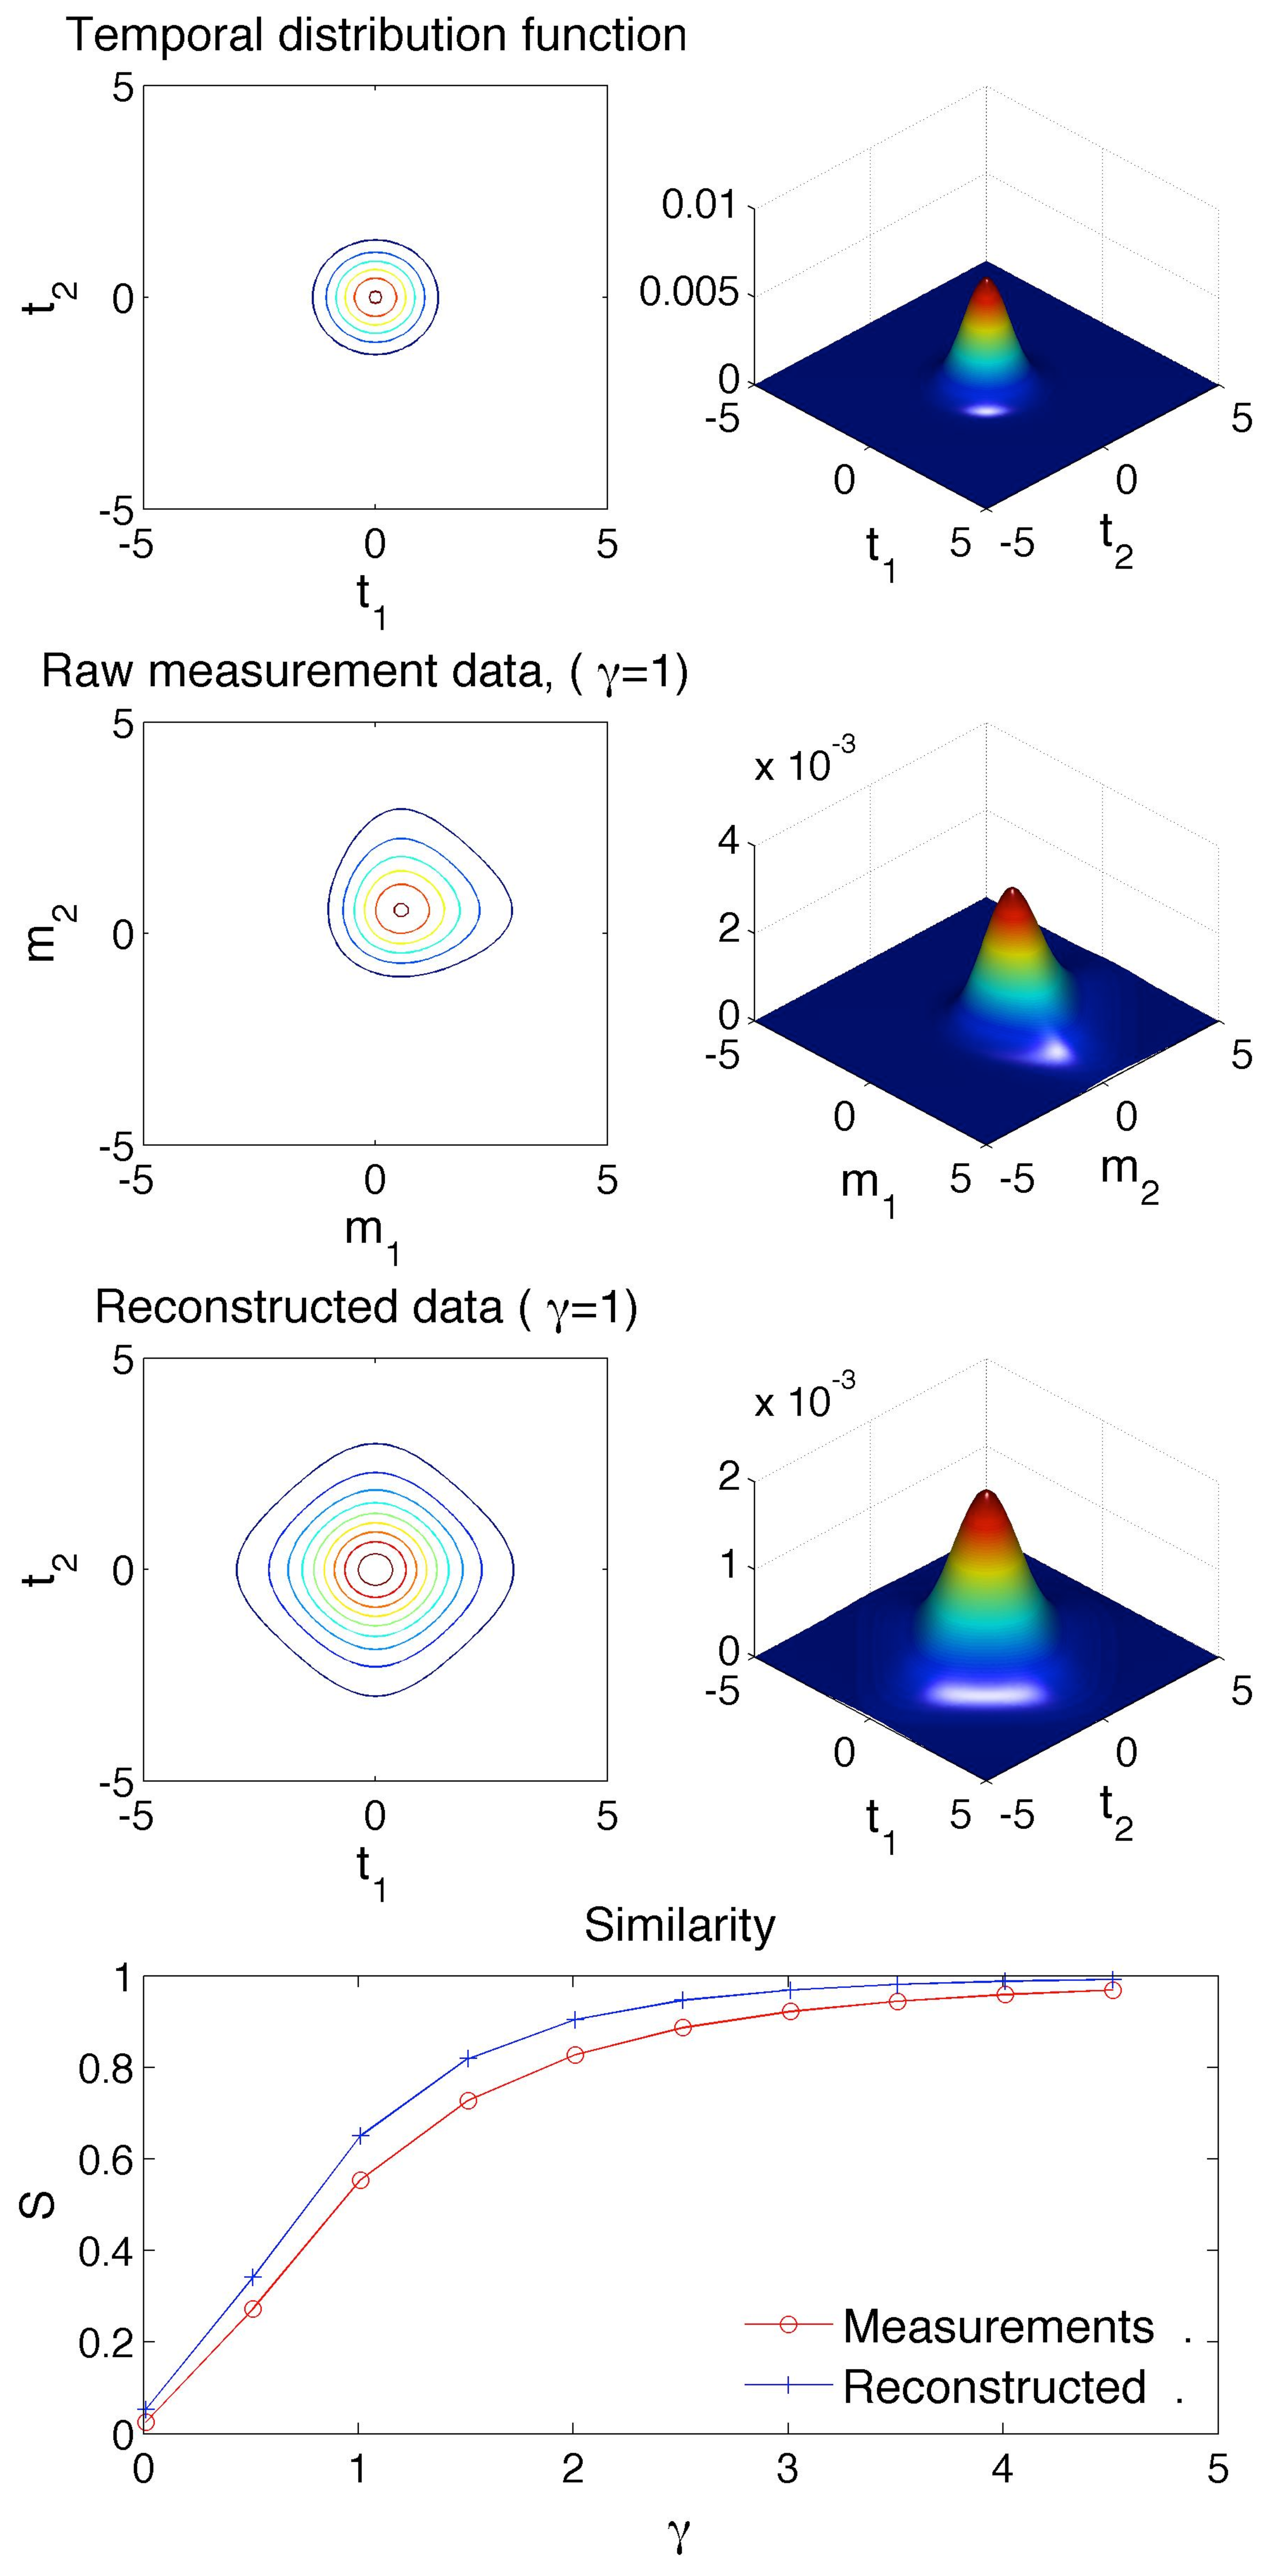
\includegraphics[width=\columnwidth]{../figures/composite_fock}
\caption{(Colour online) (a) Temporal distribution function for a two-photon Fock state. (b) Raw measurement data obtained from sampling the temporal distribution function using the photo-detectors. (c) Reconstruction based on the Bayesian algorithm. (d) Similarity of the measurement data and reconstructed data compared to the actual temporal distribution function, against detector response time $\gamma$.} \label{fig:composite_fock}
\end{figure}

We will first consider the TDF,
\begin{equation} \label{eq:spectral_gaussian}
P_S(t_{1}, t_{2}) \propto e^{-t_{1}^{2}-t_{2}^{2}},
\end{equation}
which is separable with both photons exhibiting identical temporal structure - a two-photon Fock state. This TDF is illustrated in Fig.~\ref{fig:composite_fock}(a)

The raw measurement results ($m_1$ and $m_2$) obtained from sampling this distribution are shown in Fig.~\ref{fig:composite_fock}(b). Note the asymmetry introduced into the raw data, which arises from the asymmetric response function of the photo-detectors, shown in Fig~\ref{fig:detector_response}.

The reconstruction, based on Eq.~\ref{eq:reconstr}, is shown in Fig.~\ref{fig:composite_fock}(c) for \mbox{$\gamma=1$}. Note that the reconstruction has eliminated the asymmetry introduced by the detectors. Nonetheless, the reconstruction appears diffused with the peaks being less distinct than the original TDF. This owes to the large width of the detector response function when \mbox{$\gamma=1$}. For faster detectors the peaks become more distinct and we asymptote to a perfect reconstruction (in both the cases of raw measurement data and reconstructed data).

In Fig.~\ref{fig:composite_fock}(d) we plot the similarity of the raw measurement data and reconstructed distribution (compared to the actual TDF) against the detector response time. Evidently, as the detector becomes faster (larger $\gamma$), $S$ approaches unity, whereas for slow detectors the reconstruction is very poor. The former property is because for fast detectors the detector has delta function response, thus with sufficient samples a perfect reconstruction is always obtained. Note that the reconstruction algorithm slightly improves the similarity of the inferred TDF compared to the raw measurement data.

%
% Two-photon temporal Bell state
%

\subsection{Two-photon spectral Bell state}

\begin{figure}[!htb]
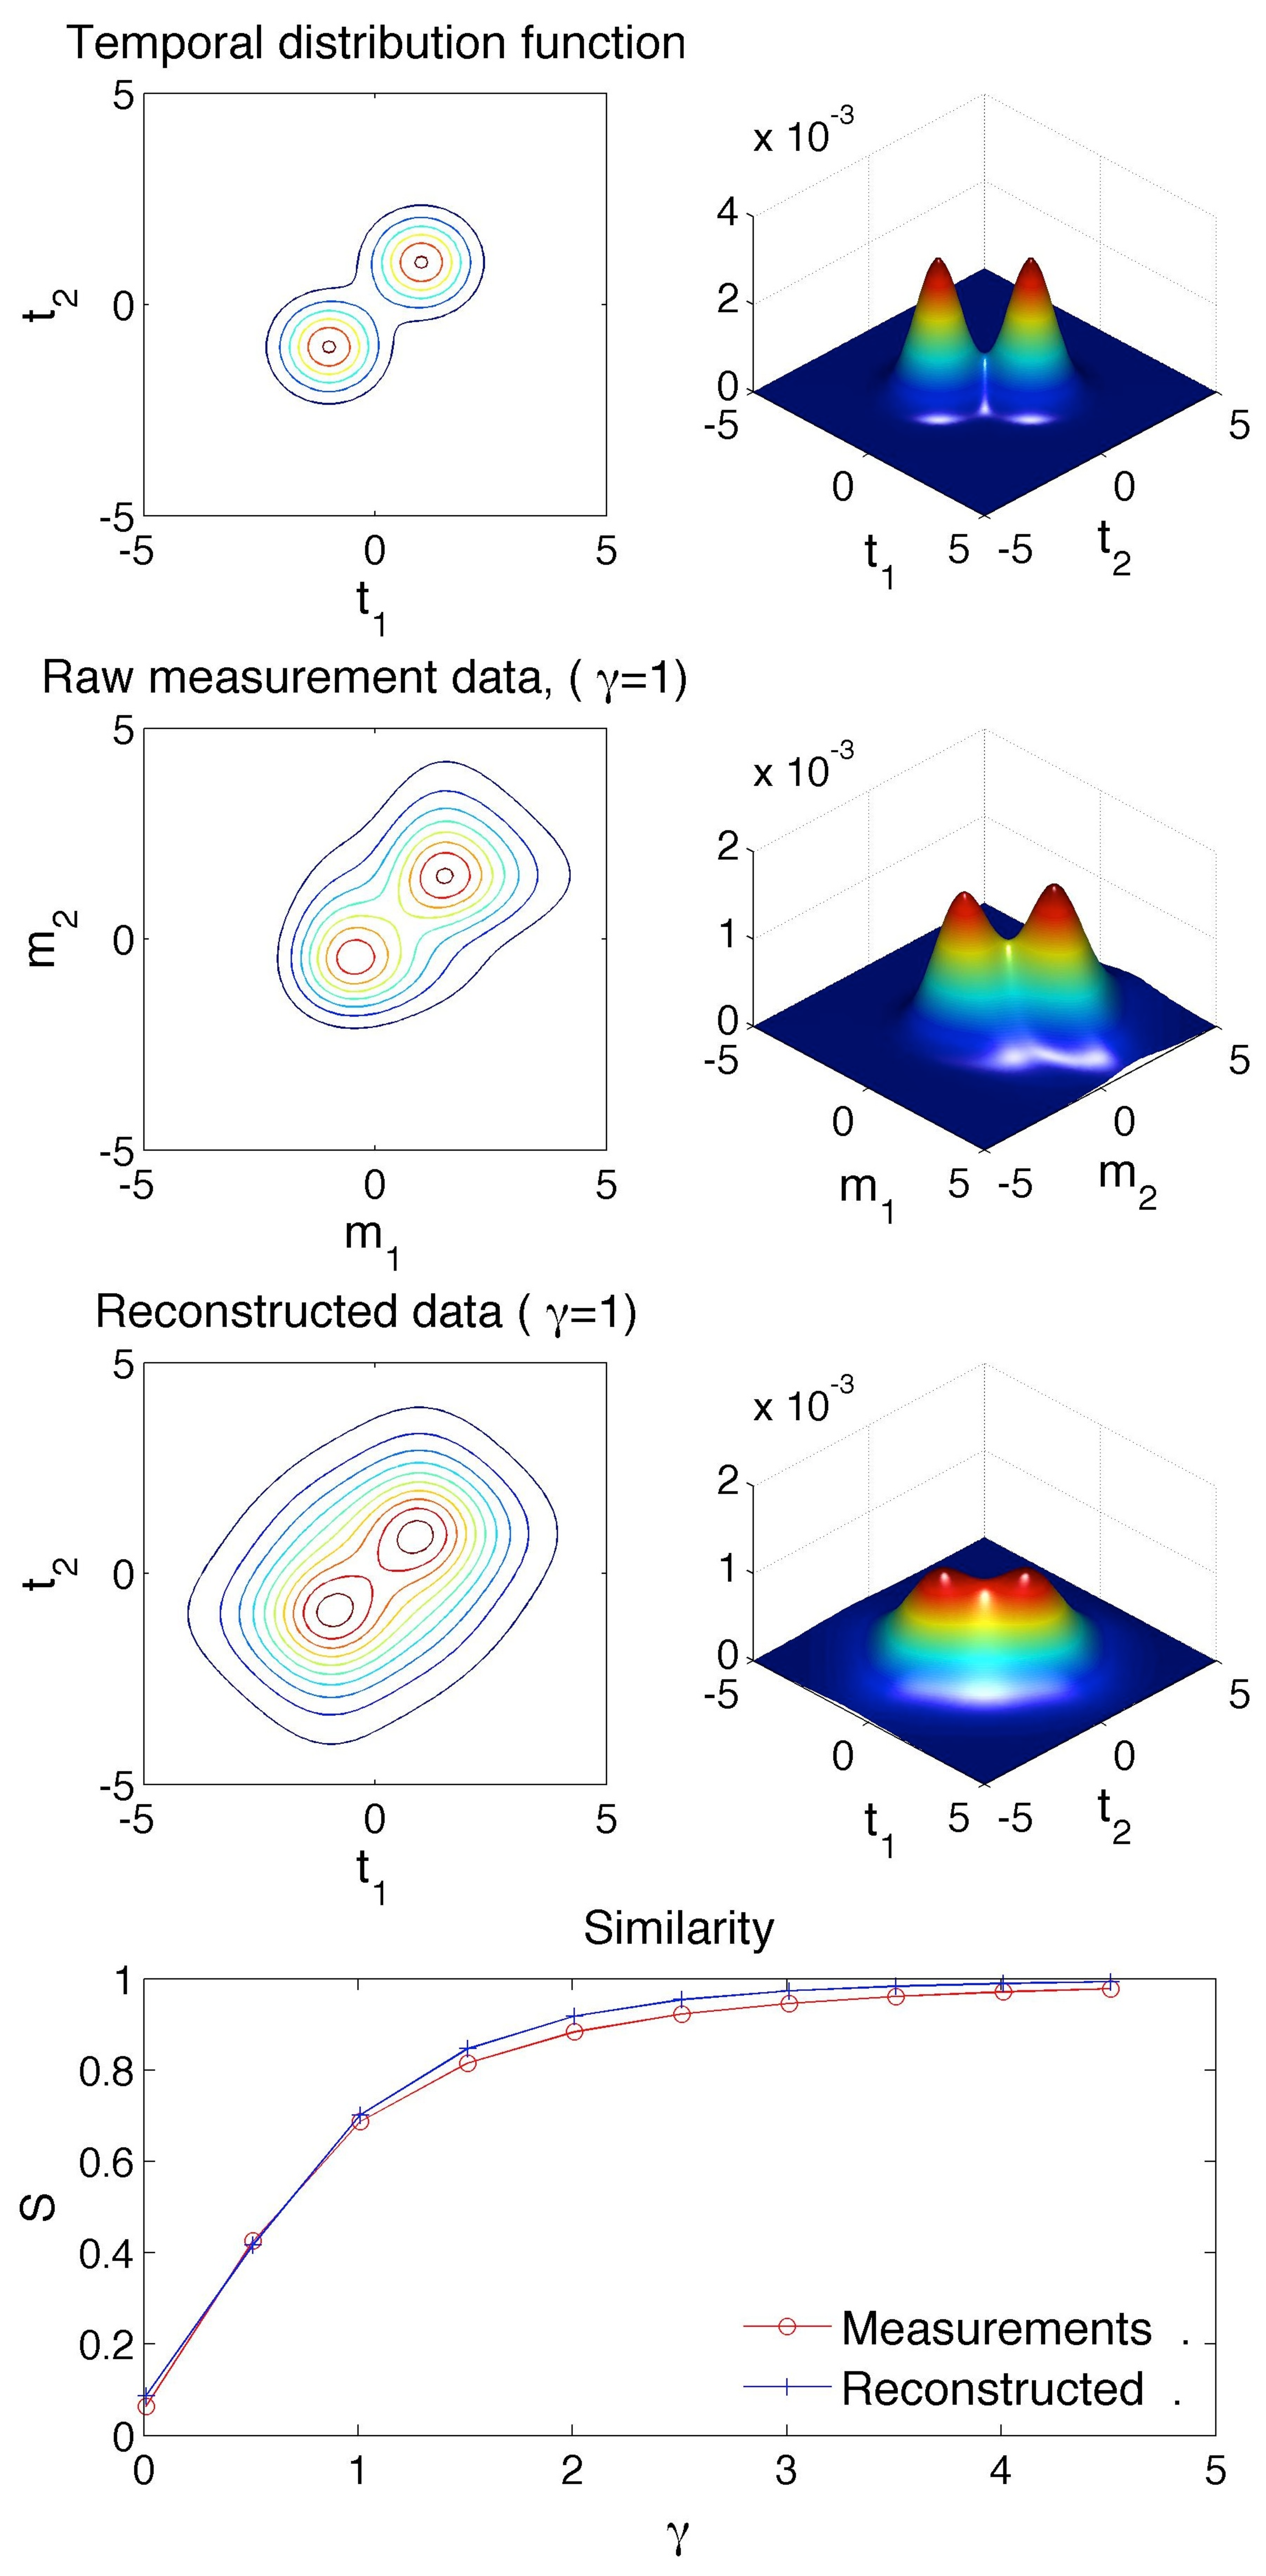
\includegraphics[width=\columnwidth]{../figures/composite_bell}
\caption{(Colour online) (a) Temporal distribution function for a Bell-like two-photon spectral state. (b) Raw measurement data obtained from sampling the temporal distribution function using the photo-detectors. (c) Reconstruction based on the Bayesian algorithm. (d) Similarity of the measurement data and reconstructed data compared to the actual temporal distribution function, against detector response time $\gamma$.} \label{fig:composite_bell}
\end{figure}

Next we consider the TDF,
\begin{equation} \label{eq:spectral_gaussian}
P_S(t_{1}, t_{2}) \propto e^{-(t_{1}-1)^{2}-(t_{2}-1)^{2}} + e^{-(t_{1}+1)^{2}-(t_{2}+1)^{2}},
\end{equation}
which has a non-separable (i.e. entangled) double-peaked Gaussian temporal structure. This is a Bell-like state, comprising two entangled Gaussian basis states. This TDF is illustrated in Fig.~\ref{fig:composite_bell}(a).

The raw measurement results are shown in Fig.~\ref{fig:composite_bell}(b). The Bayesian reconstruction is shown in Fig.~\ref{fig:composite_bell}(c) for \mbox{$\gamma=1$}.  In Fig.~\ref{fig:composite_bell}(d) we plot the similarity of the raw measurement data and reconstructed distribution (compared to the actual TDF) against the detector response time. Again we observe that the Bayesian reconstruction recovers the symmetry of the state and exhibits slightly better similarity than the raw measurement data.

%
% Parametric down-conversion states
%

\subsection{Parametric down-conversion states}

Finally we consider the spectral structure of parametric down-conversion (PDC) sources. This is of great practical interest as PDC has become the mainstay for heralded photon sources, widely used in experimental optical quantum information processing protocols. This is a two-mode device, where, when pumped with a classical field, photon pairs are produced. In the photon number basis, the output to a PDC source is of the form,
\begin{equation}
\ket{\psi}_\mathrm{PDC} = \sqrt{1-\chi^2} \sum_n \chi^n \ket{n,n}.
\end{equation}
Thus, higher order photon pair production also takes place, but we will focus on the low pump power regime (\mbox{$\chi\ll 1$}) where, upon post-selection, single pairs are dominant.

A heralded PDC source comprises a PDC source and a photo-detector. The first mode is measured, and, upon measuring a single photon, we have a single photon in the other mode with high probability. This is shown in Fig.~\ref{fig:PDC_source}.
\begin{figure}[!htb]
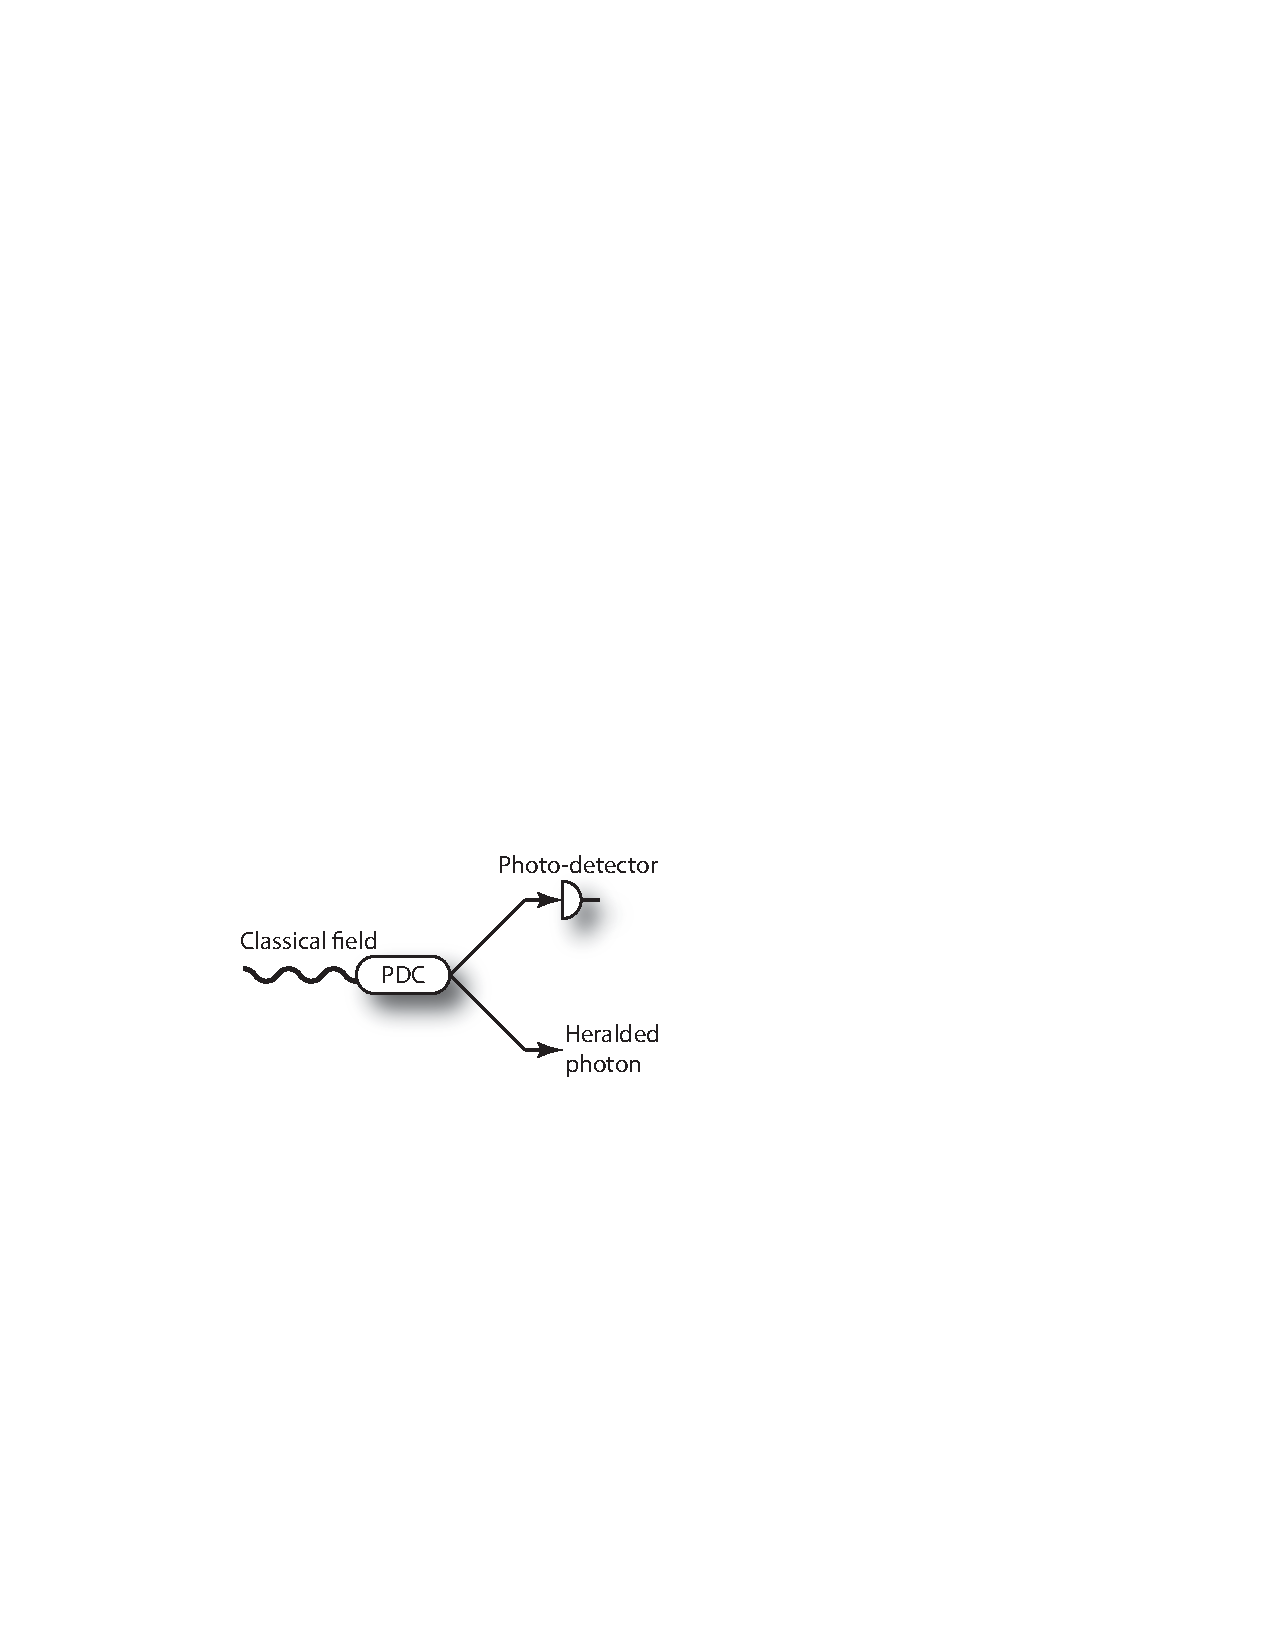
\includegraphics[width=0.6\columnwidth]{../figures/PDC_source}
\caption{Single photon source via heralded parametric down-conversion (PDC). The PDC source is pumped with a classical field and emits photon pairs across two modes. Upon performing photo-detection in one of the modes we prepare a single photon in the other.} \label{fig:PDC_source}
\end{figure}

This description is in the photon number basis. But PDC states also exhibit rich spectral structure. The full spectral/temporal description for a heralded PDC source, post-selected on a single photon pair, is of the form of Eq.~\ref{eq:multi_mode},
\begin{equation} \label{eq:PDC_spectral}
\ket{\psi}_\mathrm{PDC,PS} = \int \!\! \int \psi(t_1,t_2) \hat{a}_1^\dag(t_1) \hat{a}_2^\dag(t_2)\,dt_1 dt_2 \ket{0}.
\end{equation}

While the spectral structure of PDC states is under continuous development, and is readily manipulated via experimental parameters, as a rough approximation of realistic PDC sources, we will consider joint TDFs of the form of a rotated, asymmetric, two-dimensional Gaussian distribution,
\begin{equation} \label{eq:PDC_spectral_gaussian}
P_S(t_1,t_2) \propto e^{-(a x^2 + 2 b x y + c y^2)},
\end{equation}
where,
\begin{eqnarray}
a &=& \frac{\mathrm{cos}^2(\pi/4)}{2 w^2} + \frac{\mathrm{sin}^2(\pi/4)}{2 h^2}, \nonumber \\
b &=& -\frac{\mathrm{sin}(\pi/2)}{4 w^2} + \frac{\mathrm{sin}(\pi/2)}{4 h^2}, \nonumber \\
c &=& \frac{\mathrm{sin}^2(\pi/4)}{2 w^2} + \frac{\mathrm{cos}^2(\pi/4)}{2 h^2}.
\end{eqnarray}
This is a Gaussian distribution of width $w$ and height $h$, rotated by $\pi/4$ such that the major axis lies along the \mbox{$t_1-t_2$} plane. An example for \mbox{$h/w=5$} is shown in Fig.~\ref{fig:composite_PDC}(a). Now the height-to-width ratio, \mbox{$h/w$}, parametrises the degree of spectral entanglement.

A pressing goal for PDC development is to engineer states with separable spectral structure, such that heralding the detection of a single photon in one arms yields a highly spectrally pure single photon in the other. That is, the TDF is of the form,
\begin{equation}
\psi(t_1,t_2) = \psi_1(t_1) \cdot \psi_2(t_2).
\end{equation}
In this instance, detecting a photon in the first mode will yield a temporally pure photon in the second, with TDF given by $\psi_2(t_2)$, irrespective of the spectral/temporal properties of the photo-detection performed on the first mode. From Eq.~\ref{eq:PDC_spectral_gaussian}, this can be achieved when $h/w=1$. Otherwise the state is spectrally entangled.

While significant progress has been made in engineering spectrally separable PDC sources, most exhibit high degrees of spectral correlation (i.e. spectral entanglement). In this case a spectrally pure heralded photon will only be prepared in the presence of narrowband spectral filtering on the first mode. However, the filtering process reduces the heralding efficiency, thus engineering spectrally separable states is more desirable in terms of maximising count rates. To achieve this goal, and to characterise one's PDC sources, joint spectral tomography of the two-mode state is a pressing goal.

Steps have been made towards measuring the spectral/temporal structure of PDC states via time-delayed (i.e. HOM) interferometry \cite{bib:YoonHo03}. However, we will consider the direct approach of measurement via time-resolved photo-detection using the described reconstruction technique.

\begin{figure}[!htb]
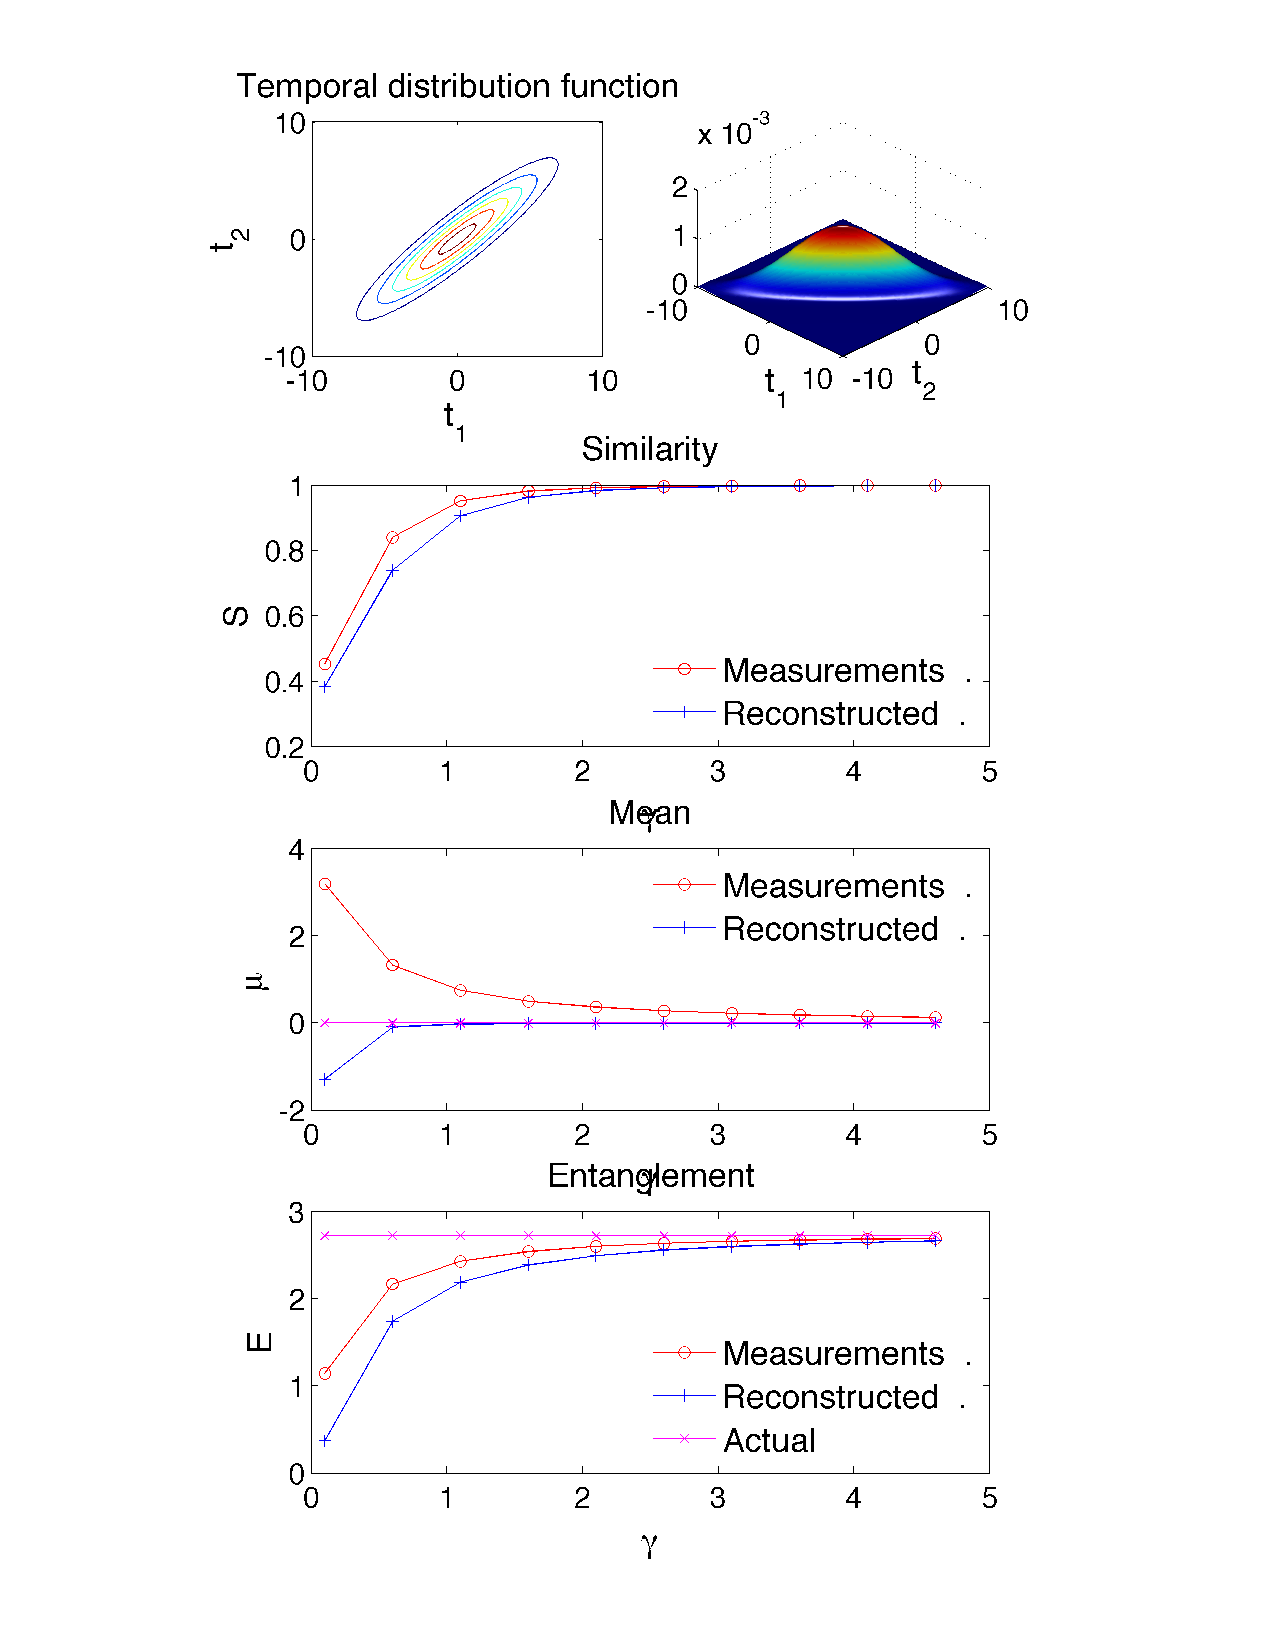
\includegraphics[width=\columnwidth]{../figures/composite_PDC}
\caption{(Colour online) (a) Temporal distribution function for a PDC photon pair (\mbox{$h/w=5$}). (b) Similarity of the measurement data and reconstructed data compared to the actual temporal distribution function, against detector response time $\gamma$. (c) Mean of the distribution. (d) Entanglement between the photons in the pair.} \label{fig:composite_PDC}
\end{figure}

In Figs.~\ref{fig:composite_PDC} \& \ref{fig:composite_PDC_3D} we plot the various quantifying measures against the height-to-width ratio of the spectral ellipsoid and detector response time, in the cases of raw measurement data and reconstructed data. Evidently, in the cases of similarity and entanglement, the raw measurement data in fact yields better outcomes than the reconstruction algorithm. On the other hand, in the case of the mean of the distribution it is evident that the reconstruction algorithm recovers the mean more accurately than the raw measurement data.

\begin{figure}[!htb]
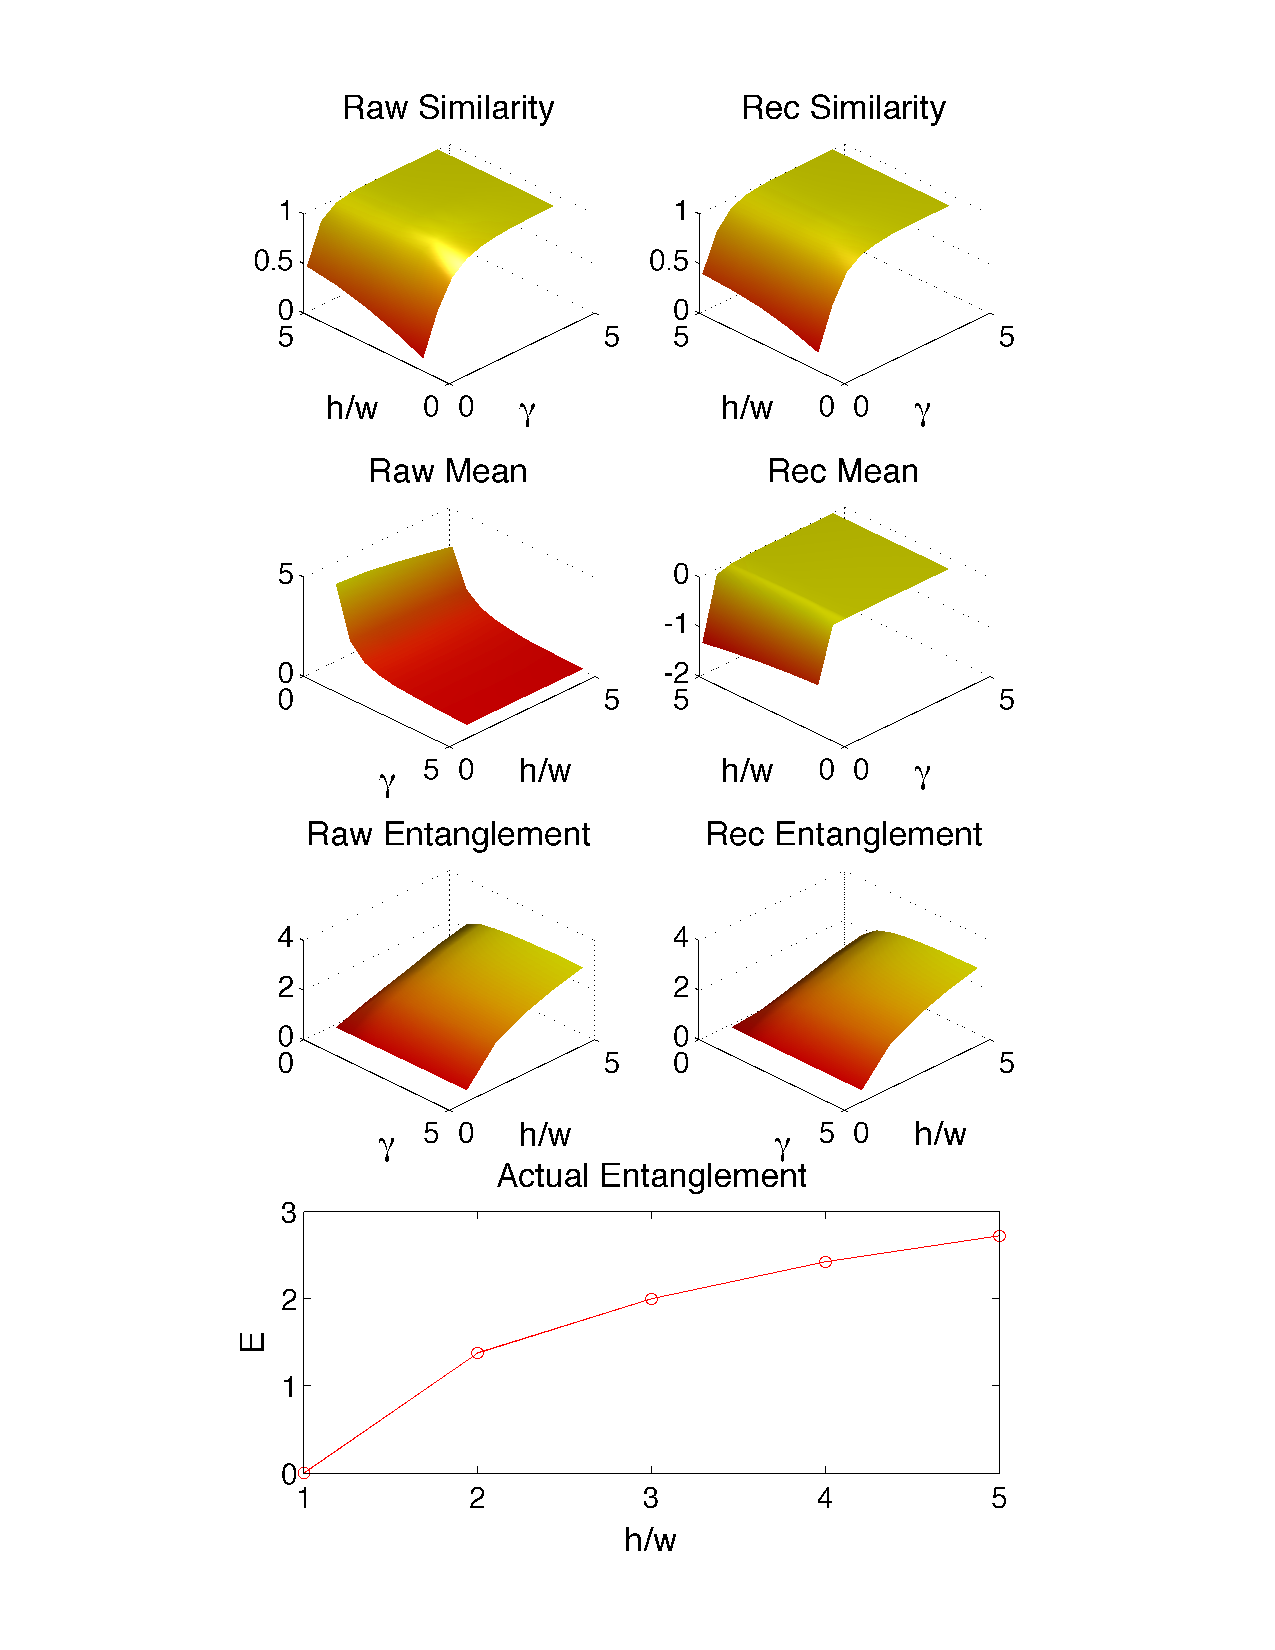
\includegraphics[width=\columnwidth]{../figures/PDC_3D}
\caption{(Colour online) (left) Raw measurement data. (right) Reconstructed data. (a) Similarity with the actual temporal distribution function. (b) Mean of the distribution (mean of actual distribution is \mbox{$\mu=0$}). (c) Spectral entanglement of the photon pair. (d) Entanglement of the actual distribution. \mbox{$h/w$} is the height-to-width ratio of the ellipsoid temporal distribution function. When \mbox{$h/w=1$} the state is spectrally separable and there is no spectral entanglement. $\gamma$ is the detector response time. Note that not all plots have the same viewing angle, so as not to obscure features.} \label{fig:composite_PDC_3D}
\end{figure}

%
% Conclusion
%

\section{Conclusion}

We have presented a tomographic procedure for characterising the spectral structure of multi-photon states, in the cases of both single- and multi-mode states. The algorithm accommodates for the temporal response of the employed photo-detectors and can improve the estimated temporal distribution function using a Bayesian approach.

The Bayesian approach was shown to improve the characterisation of the temporal structure of the photonic state compared to the raw measurement statistics.

We specifically focussed on a particular physically realistic photo-detection model. However, the techniques presented may be easily generalised to any other detector model, provided that $P_D(m|t)$ can be characterised. For example, detectors with frequency filtering, time gating or other well-defined spectral/temporal characteristics could be readily characterised in this manner. We described a simple tomographic procedure by which the temporal response of an unknown detector can be characterised.

We applied the technique to several relevant examples of spectral multi-photon states: the two-photon Fock state, the two-photon Bell state, and parametric down-conversion states.

We have specifically focussed on the temporal/spectral structure of photons. However, photons also exhibit structure in other degrees of freedom, such as spatial structure. The techniques we have described could be readily applied to such situations provided the detectors can be characterised in those domains.

%
% Acknowledgments
%

\begin{acknowledgments}
We thank Sukhi Singh for helpful discussions. This research was conducted by the Australian Research Council Centre of Excellence for Engineered Quantum Systems (Project number CE110001013).
\end{acknowledgments}

%
% Bibliography
%

\bibliography{paper}

%
% Appendix
%
\onecolumngrid
\appendix

\section{N photon states}

Consider the $n$-photon spectral state
\begin{align} \label{eq:nphotonfreq}
\ket{\psi_{N}} = \int\mathrm{d}\omega_1&\dots \mathrm{d}\omega_n \tilde\psi(\omega_1,\dots,\omega_n) a^\dag(\omega_1)\dots a^\dag(\omega_n)\ket{0}.  
\end{align}
Assuming quasi-monochromatic wave packets such that $\tilde\psi(\cdot)$ is a slowly-varying envelope with respect to the carrier frequency and $[a(\omega),a\dg(\omega')]= \delta(\omega - \omega')$.  Then, in the time domain a general $N$-photon state can be written as
\begin{align}\label{Eq::Genphoty}
\begin{split}
\ket{\psi_N} ={}\int dt_1 & \dots dt_N \, \psi(t_1,\dots,t_N)  a\dg(t_1)\dots a\dg(t_N) \ket{0}\,,%\\
\end{split}
\end{align} 
where $\psi(.)$ is the Fourier transform of $\tilde\psi(.)$.
The temporal envelope is in general neither factorable nor symmetric in $t_k$.  
 

%=======================================================
\section{Derivation of the photon counting distribution}\label{derivation}
%=======================================================
As an example of calculating the probably photon's clicking in the detectors let us consider the case where one photon clicks followed by a second photon. We will call the first click $t_1$ and the second click $t_2$. Thanks to stochastic calculus $t_1<t_2$ strictly.

\begin{align}  \label{eq:p12}
p(t_1,t_2|\psi_2)
&=  \bra{\psi_2} \Pi_J(t_2)\Pi_J(t_1)\ket{\psi_2}\\
& =\bra{\{0\}} \int dp \,dq \, \psi^*(r,s)  a(s) a(r)    \Big (a\dg(t_2)\outp{0}{0}a(t_2)\otimes a\dg(t_1)\outp{0}{0}a(t_1)\Big )   \int dp\, dq \, \psi(p,q)  a\dg(p) a\dg(q) \ket{\{0\}}\,. \nonumber\\
& =\bra{\{0\}} \int dp \,dq \, \psi^*(r,s)  a(s) a(r)   a\dg(t_2)a\dg(t_1)\ket{0}\ket{0}\underbrace{\bra{0}\bra{0}a(t_2)a(t_1)   \int dp\, dq \, \psi(p,q)  a\dg(p) a\dg(q) \ket{\{0\}}\,}_{Q }. \nonumber\\
\end{align} 
\begin{align}
Q 
&=\,_{t_2}\bra{0}_{t_1}\bra{0}a(t_2)a(t_1)   \int dp\, dq \, \psi(p,q)  a\dg(p) a\dg(q) \ket{\{0\}}\\
&=\,_{t_2}\bra{0}_{t_1}\bra{0}a(t_2)   \int dp\, dq \, \psi(p,q)  [a\dg(p)a(t_1) +\delta(t_1-p)] a\dg(q) \ket{\{0\}} \\
&=\,_{t_2}\bra{0}_{t_1}\bra{0}a(t_2)   \int dp\, dq \, \psi(p,q)  [a\dg(p)a(t_1)a\dg(q) +\delta(t_1-p)a\dg(q)]  \ket{\{0\}} \\
&=\,_{t_2}\bra{0}_{t_1}\bra{0}a(t_2)   \int dp\, dq \, \psi(p,q)  [a\dg(p)a\dg(q)a(t_1) + a\dg(p)\delta(t_1-q) +\delta(t_1-p)a\dg(q)]  \ket{\{0\}} \\
&=\,_{t_2}\bra{0}_{t_1}\bra{0}a(t_2)   \int dp\, dq \, \psi(p,q)  [ a\dg(p)\delta(t_1-q) +\delta(t_1-p)a\dg(q)]  \ket{\{0\}} \\
&=\,_{t_2}\bra{0}_{t_1}\bra{0}a(t_2)   \int dp\, dq \, \psi(p,q)   a\dg(p)\delta(t_1-q) + \int dp\, dq \, \psi(p,q) \delta(t_1-p)a\dg(q)]  \ket{\{0\}} \\
&=\,_{t_2}\bra{0}_{t_1}\bra{0}a(t_2)   \int_{t_1}^{\infty} dp\, \psi(p,t_1)   a\dg(p) + \int_{t_1}^{\infty} dq \, \psi(t_1,q) a\dg(q)]  \ket{\{0\}} \\
&=\,_{t_2}\bra{0}_{t_1}\bra{0}   \int_{t_1}^{\infty} dp\, \psi(p,t_1)  a(t_2) a\dg(p) + \int_{t_1}^{\infty} dq \, \psi(t_1,q) a(t_2)a\dg(q)]  \ket{\{0\}} \\
&=\,_{t_2}\bra{0}_{t_1}\bra{0}   \int_{t_1}^{\infty} dp\, \psi(p,t_1)  [ a\dg(p)a(t_2)+\delta(t_2-p)] + \int_{t_1}^{\infty} dq \, \psi(t_1,q) [a\dg(q)a(t_2)+\delta(t_2-q)]\ket{\{0\}} \\
&= \psi(t_2,t_1)  +  \psi(t_1,t_2)
\end{align} 
After combining this result along with its complex conjugate back into eq. \ref{eq:p12} we obtain,
\begin{align}
p(t_1,t_2|\psi_2)
&= \left[  \psi^*(t_2,t_1)  +  \psi^*(t_1,t_2)  \right] \left[  \psi(t_2,t_1)  +  \psi(t_1,t_2)  \right]\\
&= |\psi(t_2,t_1)|^2  +  \psi^*(t_1,t_2)\psi(t_2,t_1)  +
\psi^*(t_2,t_1) \psi(t_1,t_2)  +   |\psi(t_1,t_2)|^2 
\end{align}

%===================================================
\subsection{Probability for N-photons clicking}
%===================================================
This result generalises easily with Wick's theorem \cite{bib:wrcx1950evaluation} which tells us that the probabability of getting an N-photon click is the sum over all permutations,
\begin{align} \label{eq.pN}
p(t_1,t_2,t_3, \ldots, t_N|\psi_N)
=&  \left[  \sum_{\sigma\in S_N} \psi^*\big(\sigma(t_1,t_2,t_3,\ldots, t_N) \big)  \right] \left[  \sum_{\sigma\in S_N} \psi\big (\sigma(t_1,t_2,t_3,\ldots, t_N) \big)  \right],
\end{align}
where $S_N$ is the symmetric group and assuming $t_1<t_2<t_3\ldots <t_N$. Since we are dealing with photon's, which are bosons, each possible permutation is equal to each other. Then eq. \ref{eq.pN} becomes,
\begin{align}
p(t_1,t_2,t_3, \ldots, t_N|\psi_N)
=& (N!)^2   |\psi\big(t_1,t_3,t_3,\ldots, t_N \big)|^2
\end{align}

\end{document}
